\def\DoNotLoadEpstopdf{}
\documentclass[tikz,border=4pt]{standalone}
% Shared style for the technical appendix figures (2026-10-26).
% Builds on the proposal's figstyle.tex (same fonts, colors, and box styles) and adds
% one encoding for development status, used the same way in every appendix figure.
%   built and tested   solid border (the proposal's normal box styles)
%   built, no test     solid border, and the box text says "no test"
%   specified          dashed border            -> add the key  spec
%   planned            dotted grey border        -> use the style planned
%   no code (by hand)  dotted arrow              -> add the key  byhand
%   outside the artifact  solid grey border      -> use the style outside
% Shared style for proposal figures (2026-10-22 visuals pass).
% Sized to print at 6.5 in (16.5 cm) wide; body text 9 pt sans, nothing below 8 pt.
\usepackage[T1]{fontenc}
\usepackage[scaled=0.95]{helvet}
\renewcommand{\familydefault}{\sfdefault}
\usepackage{xcolor}
\usetikzlibrary{arrows.meta,positioning,calc,patterns.meta}
\definecolor{cink}{HTML}{16191F}
\definecolor{cmuted}{HTML}{4B5563}
\definecolor{cslate}{HTML}{2F4858}
\definecolor{cslatefill}{HTML}{E9EFF3}
\definecolor{cbrass}{HTML}{7A5C12}
\definecolor{cbrassfill}{HTML}{F5EFDE}
\definecolor{cred}{HTML}{8C2F39}
\definecolor{credfill}{HTML}{F8E9EA}
\definecolor{cgreen}{HTML}{235C53}
\definecolor{cgreenfill}{HTML}{E3F0EC}
\definecolor{caudit}{HTML}{5B3A8E}
\definecolor{cauditfill}{HTML}{EFE9F6}
\definecolor{cghost}{HTML}{6B7280}
\definecolor{cghostfill}{HTML}{F3F4F6}
\tikzset{
  >={Triangle[length=5pt,width=4.5pt]},
  box/.style={draw, rounded corners=1.5pt, line width=0.8pt, align=center, inner sep=4pt, font=\fontsize{9}{11}\selectfont},
  sub/.style={font=\fontsize{8}{9.6}\selectfont, text=cmuted},
  ai/.style={box, draw=cbrass, fill=cbrassfill, text=cbrass},
  ver/.style={box, draw=cred, fill=credfill, text=cred},
  pipe/.style={box, draw=cslate, fill=cslatefill, text=cslate},
  prod/.style={box, draw=cslate, fill=cslate, text=white},
  person/.style={box, draw=cink, fill=white, text=cink},
  ghost/.style={box, draw=cghost, fill=cghostfill, text=cghost, dash pattern=on 3pt off 2pt},
  flow/.style={->, line width=0.8pt},
}

\renewcommand{\ttdefault}{lmtt}% vector typewriter font (same design as the default, not a bitmap)
\tikzset{
  spec/.style={dash pattern=on 3pt off 2pt},
  planned/.style={box, draw=cghost, fill=cghostfill, text=cghost, dash pattern=on 0.9pt off 1.6pt},
  outside/.style={box, draw=cghost, fill=white, text=cghost},
  byhand/.style={dash pattern=on 0.9pt off 1.6pt},
  prog/.style={font=\fontsize{8}{9.6}\selectfont\ttfamily},
  legendbox/.style={draw, rounded corners=1pt, line width=0.8pt, minimum width=0.55cm, minimum height=0.32cm, inner sep=0pt},
  legendtext/.style={font=\fontsize{8}{9.6}\selectfont, text=cink, anchor=west, inner sep=1pt},
}
% \statuslegend{x}{y} draws the four-item status legend with its left edge at (x,y).
\newcommand{\statuslegend}[2]{%
  \begin{scope}[shift={(#1,#2)}]
    \node[legendbox, draw=cink, fill=white] (lg1) at (0.275,0) {};
    \node[legendtext] at (0.65,0) {Built and tested};
    \node[legendbox, draw=cink, fill=white, spec] (lg2) at (3.35,0) {};
    \node[legendtext] at (3.725,0) {Specified};
    \node[legendbox, draw=cghost, fill=cghostfill, dash pattern=on 0.9pt off 1.6pt] (lg3) at (5.75,0) {};
    \node[legendtext] at (6.125,0) {Planned};
    \node[legendbox, draw=cghost, fill=white] (lg4) at (7.85,0) {};
    \node[legendtext] at (8.225,0) {Outside the research artifact};
  \end{scope}}

% Figure A6 of the 10/31 appendix: how one AI contribution goes from recorded to an item of a
% verification report, followed for the AI-added citation r08 @nakamura2020 in the seeded
% references test files (verification_procedures/fixtures/citations/seeded/: citation_provenance.yaml,
% draft.md, metadata_cache.json, recorded_judge.json, source_nakamura2020.txt) and the expected
% report (tests/golden/citations_seeded/report.md), under citations.yaml 0.2.
\begin{document}
\hyphenpenalty=10000
\frenchspacing
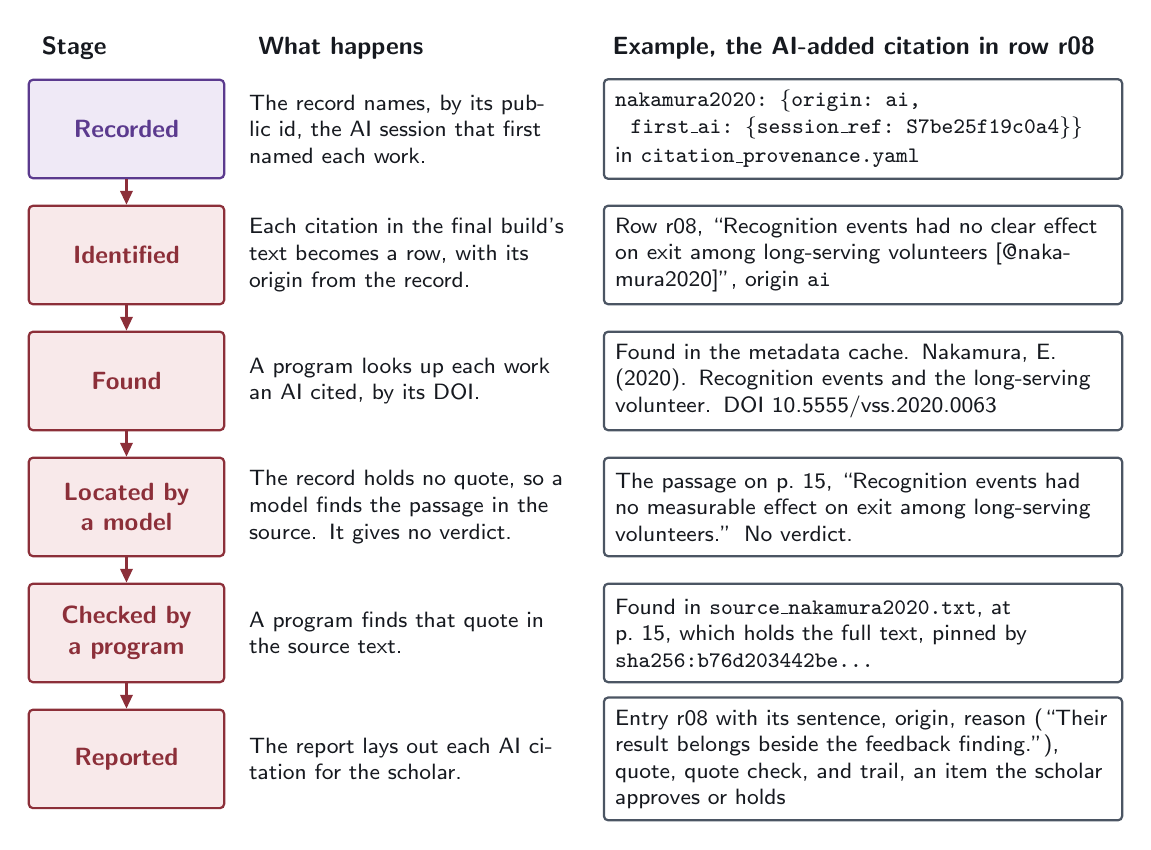
\begin{tikzpicture}
\tikzset{
  col/.style={font=\fontsize{9}{11}\selectfont\bfseries, text=cink, anchor=base west},
  stage/.style={box, text width=2.2cm, minimum width=2.4cm, minimum height=1.25cm, font=\fontsize{9}{11}\selectfont\bfseries},
  aud/.style={draw=caudit, fill=cauditfill, text=caudit},
  what/.style={anchor=west, text width=4.1cm, align=left, font=\fontsize{8}{9.6}\selectfont, text=cink, inner sep=0pt},
  ex/.style={box, anchor=west, draw=cmuted, fill=white, text=cink, text width=6.3cm, minimum width=6.5cm, minimum height=1.25cm, align=left, font=\fontsize{8}{9.6}\selectfont, inner sep=4pt},
}
\newcommand{\cd}[1]{{\fontsize{8}{9.6}\selectfont\ttfamily #1}}
\node[col] at (0.1,0.55) {Stage};
\node[col] at (2.85,0.55) {What happens};
\node[col] at (7.35,0.55) {Example, the AI-added citation in row r08};
% stages
\node[aud, stage] (s1) at (1.3,-0.4) {Recorded};
\node[ver, stage] (s2) at (1.3,-2.0) {Identified};
\node[ver, stage] (s3) at (1.3,-3.6) {Found};
\node[ver, stage] (s4) at (1.3,-5.2) {Located by a model};
\node[ver, stage] (s5) at (1.3,-6.8) {Checked by a program};
\node[ver, stage] (s6) at (1.3,-8.4) {Reported};
\foreach \a/\b in {s1/s2, s2/s3, s3/s4, s4/s5, s5/s6} {\draw[flow, cred] (\a.south) -- (\b.north);}
% what happens
\node[what] at (2.85,-0.4) {The record names, by its public id, the AI session that first named each work.};
\node[what] at (2.85,-2.0) {Each citation in the final build's text becomes a row, with its origin from the record.};
\node[what] at (2.85,-3.6) {A program looks up each work an AI cited, by its DOI.};
\node[what] at (2.85,-5.2) {The record holds no quote, so a model finds the passage in the source. It gives no verdict.};
\node[what] at (2.85,-6.8) {A program finds that quote in the source text.};
\node[what] at (2.85,-8.4) {The report lays out each AI citation for the scholar.};
% example
\node[ex] at (7.35,-0.4) {\cd{nakamura2020: \{origin: ai,}\\\cd{\ \ first\_ai: \{session\_ref: S7be25f19c0a4\}\}}\\[1pt]in \cd{citation\_provenance.yaml}};
\node[ex] at (7.35,-2.0) {Row r08, ``Recognition events had no clear effect on exit among long-serving volunteers [@nakamura2020]'', origin \cd{ai}};
\node[ex] at (7.35,-3.6) {Found in the metadata cache. Nakamura, E. (2020). Recognition events and the long-serving volunteer. DOI 10.5555/vss.2020.0063};
\node[ex] at (7.35,-5.2) {The passage on p.\ 15, ``Recognition events had no measurable effect on exit among long-serving volunteers.'' No verdict.};
\node[ex] at (7.35,-6.8) {Found in \cd{source\_nakamura2020.txt}, at p.\ 15, which holds the full text, pinned by \cd{sha256:b76d203442be...}};
\node[ex] at (7.35,-8.4) {Entry r08 with its sentence, origin, reason (``Their result belongs beside the feedback finding.''), quote, quote check, and trail, an item the scholar approves or holds};
\end{tikzpicture}
\end{document}
